\section{Case Study: The situation in Greece}
We ask participants how they assess the situation in Greece.  We examine Greece in detail for many reasons. Among the borrower countries Greece received by far the 
highest volume of loans and was most severely affected by the European debt crisis. Hence, the crisis in Greece was by far the most salient and widely debated. 
The \textit{aid$&$reform} gave rise to protests in Greece. Also Greece is the only borrower country which has not yet repaid its loans. 
In question 6 we ask, similar to question 4, which party benefited most from loans
to Greece. Again, we expect a nation-serving bias between citizens from borrower
and lender countries. The resistance of the population in Greece was large and the consequences for the population were drastic. This might give rise to a higher level of agreement between borrower and lender countries alike that the lender countries
were the main beneficiaries of the rescue program to Greece causing the divergence in opinions between lender and borrower countries to 
disappear. However, it is also conceivable that there is some level of solidarity between other lender countries and Greece causing 
the divergences to remain largely constant. We ask whether Greece will repay outstanding debt. According to 
our nation-serving hypothesis we would expect citizens from Greece (and potentially other borrower countries) to have a higher degree of confidence 
regarding the repayment of the outstanding level of debt than respondents from lender countries. \autoref{fig:figure10}

\begin{figure}[h!]
    \caption{The situation in Greece}
\begin{center}
    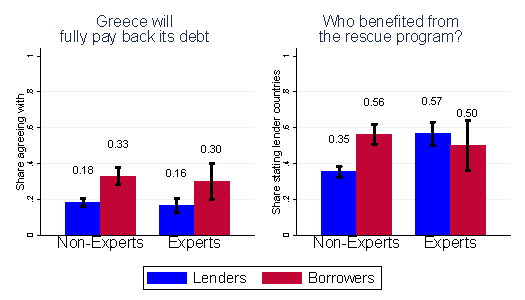
\includegraphics[scale=1.2]{graph6.pdf}

    \label{fig:figure10}
    \end{center}
    \tiny
    \begin{tablenotes}
     {The exact wording of the questions is: The two remaining questions are specifically about Greece. Question 6: Greece will fully pay back it's debt ; Answer options strongly agree, slightly agree, slightly disagree, strongly disagree, I don't know
    Question 7: Who primarily benefited from the loans granted to Greece; Answer options:  Greece, The lender countries, Both benefited equally, I don't know. We exclude all participants that answered the question with I don't know. \\
    The whiskers represent the 95 \% confidence intervals. }
    \end{tablenotes} 
\end{figure}


The results show both non-experts and experts from borrower countries (0.33 and 0.30) believe to a larger extent than non-experts and experts from lender countries (0.18 and 0.16) that Greece will fully pay its debt; a result that indicates a nation-serving bias. The observed differences are statistically significant for the sample of non-experts and experts.  

 \clearpage
 The results also show that the fraction of non-experts from lender countries (0.35) is much smaller than the fraction of non-experts from borrower countries (0.56) believing that Greece benefited from the rescue program. Inferences based on the unconditional correlations in Figure 10 are corroborated by the conditional correlations reported in Figure 11.
 NIKLAS: WAS wollen wir mit diesem ERGEBNIS MACHEN? 
 \\
\begin{figure}[h!] 
\begin{center}
     \caption{Situation in Greece}
     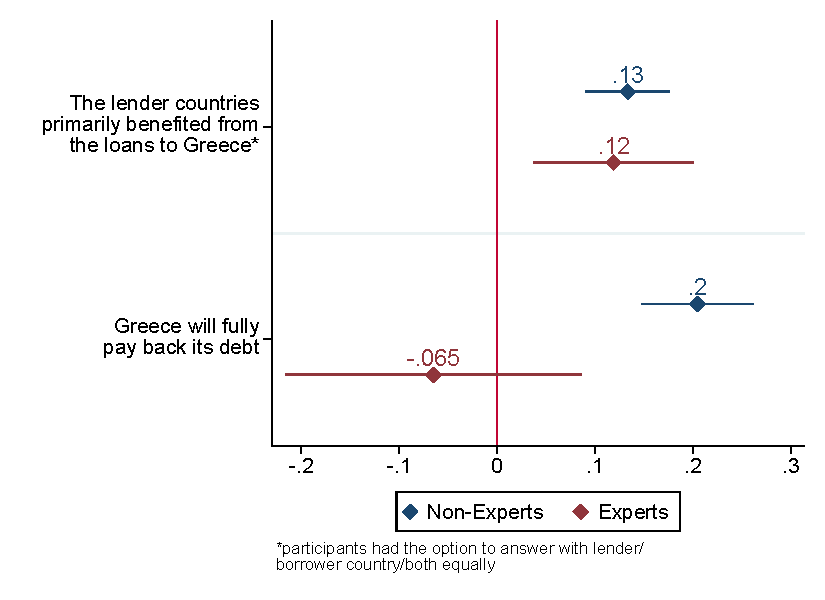
\includegraphics[scale=0.8]{Question6_7_base.pdf}
     \label{fig:my_label}
     \end{center}
     \tiny
     \tablenotes{The exact wording of the question is.   Question 6: Who primarily benefited from the loans to Greece; Question 7: Greece will fully pay back it's debt}
\end{figure}